\begin{tabular}[ht]{M{2.5cm}M{5.cm}M{5.cm}N}
  %\setlength\extrarowheight{2.5pt}
  \hline
  Particles in cells & \multicolumn{2}{c}{Critical Courant number $\frac{a\Delta t}{\Delta X}(a/b)$}  & \\[0.5cm]
   &  DCU & CTU & \\
%   & & \multicolumn{2}{c}{$a/b=1$} & \multicolumn{2}{c}{$a/b=10$} & \multicolumn{2}{c}{$a/b=1$} & \multicolumn{2}{c}{$a/b=10$}\\
   % Particles & Position of particles in cell $c$ &  \multicolumn{2}{c}{DCU} & \multicolumn{2}{c}{DCU} \\
  \hline
  \hline
  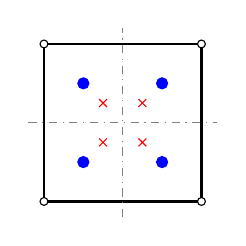
\begin{tikzpicture}[scale=1.]
    \draw[black,thick] (-1.,-1.) rectangle (1.,1.);
    \draw[black!50,dashdotted] (-1.2,0.) -- (1.2,0.0);\draw[black!50,dashdotted] (.0,-1.2) -- (0.,1.2);
    %% nodes
    \fill[white] (-1,-1) circle (0.05);\draw (-1,-1) circle (0.05);
    \fill[white] (1.,-1) circle (0.05);\draw (1,-1) circle (0.05);
    \fill[white] (1,1) circle (0.05);\draw (1,1) circle (0.05);
    \fill[white] (-1.,1) circle (0.05);\draw (-1,1) circle (0.05);
    %% particles
    \draw[Blue,mark=*] plot coordinates {(-0.5,-0.5)};
    \draw[Blue,mark=*] plot coordinates {(0.5,0.5)};
    \draw[Blue,mark=*] plot coordinates {(-0.5,0.5)};
    \draw[Blue,mark=*] plot coordinates {(0.5,-0.5)};
    %\draw[Blue,|-|] (0.5,-0.5) -- (0.5,0.5) node [midway,right] {\scriptsize $\frac{\Delta X}{2}$};
    \draw[Red,mark=x] plot coordinates {(-0.25,-0.25)};
    \draw[Red,mark=x] plot coordinates {(0.25,0.25)};
    \draw[Red,mark=x] plot coordinates {(-0.25,0.25)};
    \draw[Red,mark=x] plot coordinates {(0.25,-0.25)};
    %\draw[Red,|-|] (-0.25,-0.25) -- (-0.25,0.25) node [midway,left] {\scriptsize $\frac{\Delta X}{4}$};
  \end{tikzpicture} & 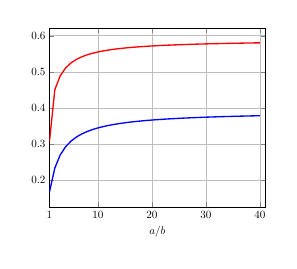
\begin{tikzpicture}[scale=0.4]
\begin{axis}[xlabel=$a/b$,ymajorgrids=true,xmajorgrids=true,xmin=1,xmax=41,xtick={1,10,20,30,40}]
%%%%%%%%%%% NATURAL CONFIGURATION
\addplot[Blue,very thick] coordinates {(1.0,0.166666666667) (2.0,0.233766233766) (3.0,0.27) (4.0,0.292682926829) (5.0,0.308219178082) (6.0,0.319526627219) (7.0,0.328125) (8.0,0.33488372093) (9.0,0.340336134454) (10.0,0.344827586207) (11.0,0.348591549296) (12.0,0.351791530945) (13.0,0.354545454545) (14.0,0.356940509915) (15.0,0.359042553191) (16.0,0.360902255639) (17.0,0.362559241706) (18.0,0.36404494382) (19.0,0.365384615385) (20.0,0.366598778004) (21.0,0.367704280156) (22.0,0.368715083799) (23.0,0.369642857143) (24.0,0.370497427101) (25.0,0.371287128713) (26.0,0.372019077901) (27.0,0.372699386503) (28.0,0.373333333333) (29.0,0.373925501433) (30.0,0.374479889043) (31.0,0.375) (32.0,0.375488917862) (33.0,0.375949367089) (34.0,0.376383763838) (35.0,0.376794258373) (36.0,0.377182770664) (37.0,0.377551020408) (38.0,0.377900552486) (39.0,0.378232758621) (40.0,0.378548895899) };
%%%%%%%%%%% MODIFIED CONFIGURATION
\addplot[Red,very thick] coordinates {(1.0,0.30612244898) (2.0,0.450574712644) (3.0,0.488913525499) (4.0,0.510638297872) (5.0,0.524625267666) (6.0,0.534383520145) (7.0,0.541578947368) (8.0,0.547103977669) (9.0,0.551479783243) (10.0,0.555031149707) (11.0,0.557971014493) (12.0,0.560444797458) (13.0,0.562555195761) (14.0,0.564376799671) (15.0,0.565965092402) (16.0,0.567362199976) (17.0,0.568600682594) (18.0,0.569706103994) (19.0,0.570698814875) (20.0,0.571595217265) (21.0,0.572408677916) (22.0,0.57315019938) (23.0,0.57382892057) (24.0,0.574452495319) (25.0,0.575027382256) (26.0,0.575559069347) (27.0,0.576052249637) (28.0,0.576510960151) (29.0,0.576938692651) (30.0,0.577338482686) (31.0,0.577712981744) (32.0,0.578064516129) (33.0,0.578395135328) (34.0,0.578706652) (35.0,0.579000675219) (36.0,0.579278638279) (37.0,0.579541822056) (38.0,0.579791374747) (39.0,0.580028328612) (40.0,0.58025361425) };
\end{axis}
\end{tikzpicture}
%%% Local Variables:
%%% mode: latex
%%% TeX-master: "../../mainManuscript"
%%% End:
 & 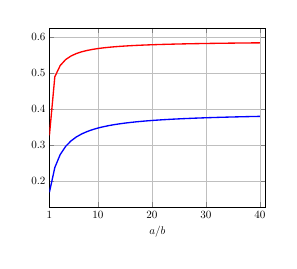
\begin{tikzpicture}[scale=0.4]
\begin{axis}[xlabel=$a/b$,ymajorgrids=true,xmajorgrids=true,xmin=1,xmax=41,xtick={1,10,20,30,40}]
%%%%%%%%%%% NATURAL CONFIGURATION
\addplot[Blue,very thick] coordinates {(1.0,0.167891991267) (2.0,0.236676134687) (3.0,0.272980739363) (4.0,0.295523052838) (5.0,0.31086679909) (6.0,0.321980387453) (7.0,0.330399242911) (8.0,0.336996589796) (9.0,0.342305428681) (10.0,0.346669420492) (11.0,0.350320058356) (12.0,0.353418957124) (13.0,0.356082359353) (14.0,0.358396007915) (15.0,0.360424530234) (16.0,0.362217559503) (17.0,0.363813843724) (18.0,0.36524407401) (19.0,0.366532874772) (20.0,0.367700231858) (21.0,0.368762535467) (22.0,0.369733353839) (23.0,0.370624015434) (24.0,0.371444052722) (25.0,0.372201544487) (26.0,0.372903382721) (27.0,0.373555482814) (28.0,0.374162950599) (29.0,0.374730216246) (30.0,0.375261142441) (31.0,0.375759112422) (32.0,0.376227102125) (33.0,0.376667739677) (34.0,0.377083354767) (35.0,0.377476019835) (36.0,0.37784758462) (37.0,0.378199705293) (38.0,0.378533869127) (39.0,0.378851415496) (40.0,0.379153553806) };
%%%%%%%%%%% MODIFIED CONFIGURATION
\addplot[Red,very thick] coordinates {(1.0,0.326304188278) (2.0,0.489325348197) (3.0,0.520649204857) (4.0,0.537092735424) (5.0,0.547194071957) (6.0,0.554021734434) (7.0,0.558942755592) (8.0,0.56265696686) (9.0,0.565559375666) (10.0,0.567889697418) (11.0,0.56980178835) (12.0,0.571398904651) (13.0,0.572752913461) (14.0,0.573915372853) (15.0,0.57492422974) (16.0,0.575808031925) (17.0,0.57658866765) (18.0,0.577283199978) (19.0,0.577905126649) (20.0,0.578465264862) (21.0,0.578972385091) (22.0,0.579433673213) (23.0,0.579855072848) (24.0,0.580241542647) (25.0,0.580597252178) (26.0,0.580925732862) (27.0,0.581229995544) (28.0,0.581512622996) (29.0,0.58177584338) (30.0,0.582021589074) (31.0,0.58225154418) (32.0,0.582467183146) (33.0,0.58266980241) (34.0,0.582860546471) (35.0,0.583040429512) (36.0,0.583210353437) (37.0,0.583371122983) (38.0,0.583523458467) (39.0,0.583668006571) (40.0,0.583805349515) };
\end{axis}
\end{tikzpicture}
%%% Local Variables:
%%% mode: latex
%%% TeX-master: "../../mainManuscript"
%%% End:
& \\ [3.25cm]
  %%%%%%%%%%%%%%%%%%%%%%%%%%%%%%%%%%%%%%%
  %%%%%%%%%%%%%%%%%%%%%%%%%%%%%%%%%%%%%%% 
  \hline % Shifted left // Shifted right
  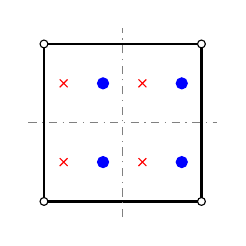
\begin{tikzpicture}[scale=1.]
    \draw[black,thick] (-1.,-1.) rectangle (1.,1.);
    \draw[black!50,dashdotted] (-1.2,0.) -- (1.2,0.0);\draw[black!50,dashdotted] (.0,-1.2) -- (0.,1.2);
    %% nodes
    \fill[white] (-1,-1) circle (0.05);\draw (-1,-1) circle (0.05);
    \fill[white] (1.,-1) circle (0.05);\draw (1,-1) circle (0.05);
    \fill[white] (1,1) circle (0.05);\draw (1,1) circle (0.05);
    \fill[white] (-1.,1) circle (0.05);\draw (-1,1) circle (0.05);
    %% particles
    \draw[Blue,mark=*] plot coordinates {(-0.5+0.25,-0.5)};
    \draw[Blue,mark=*] plot coordinates {(0.5+0.25,0.5)};
    \draw[Blue,mark=*] plot coordinates {(-0.5+0.25,0.5)};
    \draw[Blue,mark=*] plot coordinates {(0.5+0.25,-0.5)};
    \draw[Red,mark=x] plot coordinates {(-0.5-0.25,-0.5)};
    \draw[Red,mark=x] plot coordinates {(0.5-0.25,0.5)};
    \draw[Red,mark=x] plot coordinates {(-0.5-0.25,0.5)};
    \draw[Red,mark=x] plot coordinates {(0.5-0.25,-0.5)};
  \end{tikzpicture}  & 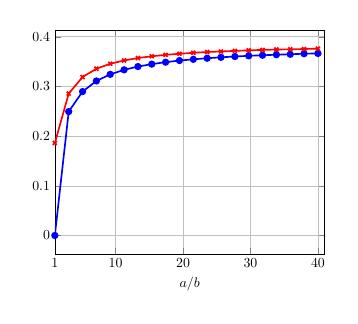
\begin{tikzpicture}[scale=0.5]
\begin{axis}[xlabel=$a/b$,ymajorgrids=true,xmajorgrids=true,xmin=1,xmax=41,xtick={1,10,20,30,40}]
%%%%%%%%%%% NATURAL CONFIGURATION
\addplot[Blue,mark=*,very thick] coordinates {(1.0,1.0000100001e-05) (3.05263157895,0.249310914162) (5.10526315789,0.28957342205) (7.15789473684,0.311013636452) (9.21052631579,0.324305874638) (11.2631578947,0.333392807612) (13.3157894737,0.339955504818) (15.3684210526,0.344870817129) (17.4210526316,0.348772961414) (19.4736842105,0.352087731404) (21.5263157895,0.354541966472) (23.5789473684,0.356753041215) (25.6315789474,0.358589375367) (27.6842105263,0.360175180699) (29.7368421053,0.361603616036) (31.7894736842,0.362721521952) (33.8421052632,0.363806269642) (35.8947368421,0.364694173258) (37.9473684211,0.365816289742) (40.0,0.366403664037) };
%%%%%%%%%%% MODIFIED CONFIGURATION
\addplot[Red,mark=x,very thick] coordinates {(1.0,0.186161861619) (3.05263157895,0.285515486734) (5.10526315789,0.318877925621) (7.15789473684,0.335565460918) (9.21052631579,0.345582403192) (11.2631578947,0.352315102098) (13.3157894737,0.357133045015) (15.3684210526,0.36070044911) (17.4210526316,0.363581004231) (19.4736842105,0.365719446668) (21.5263157895,0.367673150416) (23.5789473684,0.36925000829) (25.6315789474,0.37038001959) (27.6842105263,0.371525820521) (29.7368421053,0.372606357643) (31.7894736842,0.37353005109) (33.8421052632,0.374297427185) (35.8947368421,0.37474480008) (37.9473684211,0.375303226716) (40.0,0.376003760038) };
\end{axis}
\end{tikzpicture}
%%% Local Variables:
%%% mode: latex
%%% TeX-master: "../../mainManuscript"
%%% End:
 &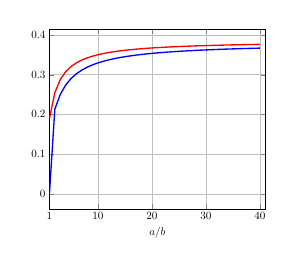
\begin{tikzpicture}[scale=0.4]
\begin{axis}[xlabel=$a/b$,ymajorgrids=true,xmajorgrids=true,xmin=1,xmax=41,xtick={1,10,20,30,40}]
%%%%%%%%%%% NATURAL CONFIGURATION
\addplot[Blue,very thick] coordinates {(1.0,-1.59364188514e-12) (2.0,0.212857320897) (3.0,0.249893924351) (4.0,0.27360416432) (5.0,0.290070593852) (6.0,0.30216822431) (7.0,0.311430129824) (8.0,0.318747857117) (9.0,0.324674954147) (10.0,0.329573175966) (11.0,0.333688883167) (12.0,0.337195633388) (13.0,0.340219213023) (14.0,0.342853009248) (15.0,0.345167807082) (16.0,0.347218235209) (17.0,0.349047125479) (18.0,0.350688533417) (19.0,0.352169876071) (20.0,0.3535134741) (21.0,0.354737683146) (22.0,0.355857736689) (23.0,0.356886382692) (24.0,0.357834370589) (25.0,0.358710828109) (26.0,0.359523555947) (27.0,0.360279260443) (28.0,0.360983738964) (29.0,0.361642028851) (30.0,0.362258527996) (31.0,0.362837093184) (32.0,0.36338112082) (33.0,0.363893613627) (34.0,0.364377236081) (35.0,0.364834360724) (36.0,0.365267107082) (37.0,0.365677374516) (38.0,0.36606687008) (39.0,0.366437132262) (40.0,0.366789551283) };
%%%%%%%%%%% MODIFIED CONFIGURATION
\addplot[Red,very thick] coordinates {(1.0,0.18887015067) (2.0,0.254459520239) (3.0,0.287403904864) (4.0,0.307169534548) (5.0,0.320334758075) (6.0,0.329729082668) (7.0,0.336768311765) (8.0,0.342238808871) (9.0,0.346612107914) (10.0,0.350188061313) (11.0,0.353166425063) (12.0,0.355685394958) (13.0,0.357843617559) (14.0,0.359713389803) (15.0,0.361348904135) (16.0,0.362791580609) (17.0,0.364073619671) (18.0,0.36522043174) (19.0,0.366252337065) (20.0,0.367185779335) (21.0,0.368034207917) (22.0,0.368808729666) (23.0,0.369518597597) (24.0,0.370171582133) (25.0,0.370774256583) (26.0,0.371332219112) (27.0,0.371850267081) (28.0,0.372332535292) (29.0,0.372782606539) (30.0,0.373203600747) (31.0,0.373598247379) (32.0,0.373968944663) (33.0,0.374317808349) (34.0,0.374646712123) (35.0,0.374957321245) (36.0,0.375251120754) (37.0,0.375529439201) (38.0,0.375793468735) (39.0,0.376044282167) (40.0,0.376282847537) };
\end{axis}
\end{tikzpicture}
%%% Local Variables:
%%% mode: latex
%%% TeX-master: "../../mainManuscript"
%%% End:
& \\ [3.25cm]
  %%%%%%%%%%%%%%%%%%%%%%%%%%%%%%%%%%%%%
  %%%%%%%%%%%%%%%%%%%%%%%%%%%%%%%%%%%%%
  \hline % Shifted above // Shifted below
  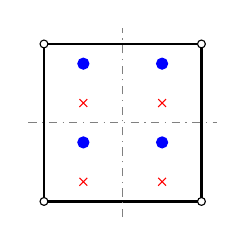
\begin{tikzpicture}[scale=1.]
    \draw[black,thick] (-1.,-1.) rectangle (1.,1.);
    \draw[black!50,dashdotted] (-1.2,0.) -- (1.2,0.0);\draw[black!50,dashdotted] (.0,-1.2) -- (0.,1.2);
    %% nodes
    \fill[white] (-1,-1) circle (0.05);\draw (-1,-1) circle (0.05);
    \fill[white] (1.,-1) circle (0.05);\draw (1,-1) circle (0.05);
    \fill[white] (1,1) circle (0.05);\draw (1,1) circle (0.05);
    \fill[white] (-1.,1) circle (0.05);\draw (-1,1) circle (0.05);
    %% particles
    \draw[Blue,mark=*] plot coordinates {(-0.5,-0.5+0.25)};
    \draw[Blue,mark=*] plot coordinates {(0.5,0.5+0.25)};
    \draw[Blue,mark=*] plot coordinates {(-0.5,0.5+0.25)};
    \draw[Blue,mark=*] plot coordinates {(0.5,-0.5+0.25)};
    \draw[Red,mark=x] plot coordinates {(-0.5,-0.5-0.25)};
    \draw[Red,mark=x] plot coordinates {(0.5,0.5-0.25)};
    \draw[Red,mark=x] plot coordinates {(-0.5,0.5-0.25)};
    \draw[Red,mark=x] plot coordinates {(0.5,-0.5-0.25)};
  \end{tikzpicture}& 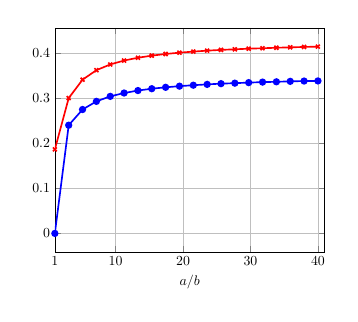
\begin{tikzpicture}[scale=0.5]
\begin{axis}[xlabel=$a/b$,ymajorgrids=true,xmajorgrids=true,xmin=1,xmax=41,xtick={1,10,20,30,40}]
%%%%%%%%%%% NATURAL CONFIGURATION
\addplot[Blue,mark=*,very thick] coordinates {(1.0,1.0000100001e-05) (3.05263157895,0.239878188256) (5.10526315789,0.274614851412) (7.15789473684,0.292689242682) (9.21052631579,0.303766195557) (11.2631578947,0.311204164673) (13.3157894737,0.316652640211) (15.3684210526,0.32074215479) (17.4210526316,0.323860607027) (19.4736842105,0.326382211191) (21.5263157895,0.328494863896) (23.5789473684,0.330344356075) (25.6315789474,0.331932266691) (27.6842105263,0.333044383075) (29.7368421053,0.334245447718) (31.7894736842,0.335382301191) (33.8421052632,0.336055465818) (35.8947368421,0.337054949497) (37.9473684211,0.337734956297) (40.0,0.338003380034) };
%%%%%%%%%%% MODIFIED CONFIGURATION
\addplot[Red,mark=x,very thick] coordinates {(1.0,0.186161861619) (3.05263157895,0.299954578493) (5.10526315789,0.340728670445) (7.15789473684,0.361763617636) (9.21052631579,0.374503745037) (11.2631578947,0.383176463344) (13.3157894737,0.389357577786) (15.3684210526,0.394050256292) (17.4210526316,0.397726608845) (19.4736842105,0.400577689987) (21.5263157895,0.402976661346) (23.5789473684,0.405090366693) (25.6315789474,0.406777225667) (27.6842105263,0.408069343851) (29.7368421053,0.409480410594) (31.7894736842,0.410406209325) (33.8421052632,0.411524115241) (35.8947368421,0.412434650662) (37.9473684211,0.413250974615) (40.0,0.414004140041) };
\end{axis}
\end{tikzpicture}
%%% Local Variables:
%%% mode: latex
%%% TeX-master: "../../mainManuscript"
%%% End:
 &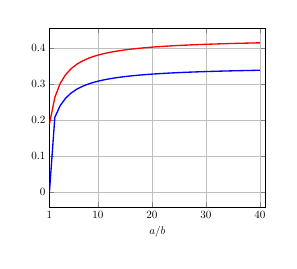
\begin{tikzpicture}[scale=0.4]
\begin{axis}[xlabel=$a/b$,ymajorgrids=true,xmajorgrids=true,xmin=1,xmax=41,xtick={1,10,20,30,40}]
%%%%%%%%%%% NATURAL CONFIGURATION
\addplot[Blue,very thick] coordinates {(1.0,-6.54115650537e-13) (2.0,0.207631685065) (3.0,0.240430029398) (4.0,0.26096289659) (5.0,0.275016910974) (6.0,0.285237324443) (7.0,0.293003101823) (8.0,0.299103117316) (9.0,0.304021109389) (10.0,0.308070133656) (11.0,0.311461709667) (12.0,0.314343883947) (13.0,0.316823369995) (14.0,0.318979027962) (15.0,0.320870393341) (16.0,0.322543253386) (17.0,0.324033398269) (18.0,0.325369207815) (19.0,0.326573474704) (20.0,0.327664714709) (21.0,0.328658124781) (22.0,0.329566294666) (23.0,0.330399742969) (24.0,0.331167326188) (25.0,0.331876554506) (26.0,0.332533838231) (27.0,0.33314468201) (28.0,0.333713839307) (29.0,0.334245436298) (30.0,0.334743072039) (31.0,0.335209900028) (32.0,0.335648695078) (33.0,0.336061908505) (34.0,0.336451713928) (35.0,0.336820045512) (36.0,0.337168630053) (37.0,0.337499014044) (38.0,0.337812586608) (39.0,0.33811059902) (40.0,0.338394181387) };
%%%%%%%%%%% MODIFIED CONFIGURATION
\addplot[Red,very thick] coordinates {(1.0,0.18887015067) (2.0,0.262956392078) (3.0,0.302076047328) (4.0,0.32618849157) (5.0,0.342522128096) (6.0,0.354312580524) (7.0,0.363221663933) (8.0,0.370189579051) (9.0,0.375787926093) (10.0,0.380384094421) (11.0,0.384224929247) (12.0,0.387482399219) (13.0,0.390279973956) (14.0,0.392708588922) (15.0,0.394836695539) (16.0,0.396716803678) (17.0,0.398389865869) (18.0,0.399888290415) (19.0,0.401238058753) (20.0,0.402460243029) (21.0,0.403572113124) (22.0,0.404587957102) (23.0,0.405519698035) (24.0,0.406377363812) (25.0,0.407169449254) (26.0,0.407903198264) (27.0,0.408584825881) (28.0,0.409219694664) (29.0,0.409812455992) (30.0,0.410367164166) (31.0,0.41088736923) (32.0,0.411376192992) (33.0,0.411836391706) (34.0,0.412270408049) (35.0,0.412680414481) (36.0,0.413068349603) (37.0,0.413435948794) (38.0,0.413784770166) (39.0,0.414116216626) (40.0,0.414431554738) };
\end{axis}
\end{tikzpicture}
%%% Local Variables:
%%% mode: latex
%%% TeX-master: "../../mainManuscript"
%%% End:
& \\ [3.25cm]
  %\begin{minipage}{0.85\textwidth}\lipsum[1]\end{minipage}
  \hline
\end{tabular}

%%% Local Variables: 
%%% mode: latex
%%% TeX-master: "../../mainManuscript"
%%% End: